\section{当前工作目录}

\begin{figure}[h!]
\centering
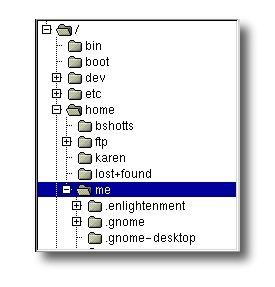
\includegraphics[width=2.5in]{images/1.png}
\caption{File system tree as shown by a graphical file manager}
\label{fig_sim}
\end{figure}

大多数人都可能熟悉图形文件管理器,它描述了文件系统树的结构,正如图1所示。 注意通常,这是一棵倒置的树,也就是说,树根在最上面,而各个枝干在下面展开。

\par 然而,命令行没有图片,所以我们需要考虑用不同的方法,在文件系统树中跳转。

\par 把文件系统想象成一个迷宫形状,就像一棵倒立的大树,我们站在迷宫的中间位置。 在任意时刻,我们处于一个目录里面,我们能看到这个目录包含的所有文件, 以及通往上面目录(父目录)的路径,和下面的各个子目录。我们所在的目录则称为 当前工作目录。我们使用 pwd(打印工作目录)命令,来显示当前工作目录。

\begin{lstlisting}
[me@linuxbox ~]$ pwd
/home/me
\end{lstlisting}

\par 当我们首次登录系统后,(或者启动终端仿真器会话后),当前工作目录设置成主目录。 每个用户都有他自己的主目录,当用户以普通用户的身份操控系统时,主目录是唯一 允许用户编写文件的地方。

